\documentclass[11pt,a4paper]{article}
\usepackage[T1]{fontenc}
\usepackage[utf8]{inputenc}
\usepackage{lmodern}
\usepackage[margin=1.85cm]{geometry}
\usepackage{amsmath,amssymb,amsthm,mathtools}
\usepackage{booktabs}
\usepackage{array}
\usepackage{graphicx}
\usepackage{microtype}
\usepackage{xcolor}
\usepackage{hyperref}

\hypersetup{
    colorlinks=true,
    linkcolor=blue!70!black,
    citecolor=blue!70!black,
    urlcolor=blue!70!black
}
\emergencystretch=1.5em

\title{\textbf{Tau Core Frontier Closures --- Part I (Pillar 1):}\\
Covariant 4D Disformal Clock-Lapse Optical Resolution of the $\theta_*$--\texttt{DESI} BAO--SN Triangle, Relativistic Swiss-Cheese Weinberg No-Go Theorem, and \texttt{Pantheon+SH0ES} Local-Void Ceiling}

\author{Jozsef Olcsak\\[0.25em]
\small Independent Researcher $\cdot$ ORCID: \href{https://orcid.org/0009-0003-7311-6522}{0009-0003-7311-6522}\\
\small Tau Core Research Program --- Paper 29 (\texttt{v1.1.0-step1})}
\date{23 November 2026}

\begin{document}
\maketitle

\begin{abstract}
\noindent Untruncated $\ell \in [2, 3000]$ Boltzmann and curved-sky Wigner-$d$ gravitational lensing calculations in Paper~28 (\texttt{v4.5.0}) established that the screened single-metric \texttt{AeST}--QUMOND Helmholtz sector of Tau Core ($\kappa_\theta = \xi_\Phi^2 = (256\pi^2)^2$, physical condensate-to-baryon ratio $R_{A/b} = (213\sqrt{3}-20)/65$, $\omega_b = 0.02240$, $\omega_m = 0.143281$, $\sum m_\nu = 0.05919\;\mathrm{eV}$, zero added parameters) reproduces both the 22-bin \texttt{ACT DR6 v1.2 + Planck PR4} lensing power spectrum ($\chi^2/\mathrm{dof} = 0.986\text{--}1.039$) and the 108-bin \texttt{ACT DR6} Silk-damped primary CMB spectra ($\chi^2/\mathrm{dof} = 1.007\text{--}1.021$) at the homogeneous $\theta_*$-locked Hubble constant $H_0^{(\theta_*)} = 67.273\;\mathrm{km\,s^{-1}\,Mpc^{-1}}$, while exposing a sharp $+0.271\%$ acoustic shift ($100\theta_* = 1.04372$) when $H_0 = 68.22\;\mathrm{km\,s^{-1}\,Mpc^{-1}}$ is imposed on a strictly homogeneous flat-FLRW background. Here, in Part~I of Paper~29, we close this optical-versus-homogeneous diagnostic under strict referee discipline across four reproducible gates (\texttt{Gates S1.1--S1.4}):
(1)~\textbf{4D Swiss-Cheese LTB Weinberg No-Go (\texttt{PROVEN NO-GO}):} Integrating 400 exact $C^2$ Darmois--Israel-matched mass-compensated Lema\^{\i}tre--Tolman--Bondi (LTB) dust+$\Lambda$ shells ($\delta_0 = -0.7833$, wall peak $+0.6110$, proper mass-compensation residual $4.54\times 10^{-6}$) together with 64 ergodic non-radial Eulerian sightlines and dimensionally exact coupled 4D Ricci/Weyl tidal-shear Sachs equations out to $z_* = 1089.983$ yields an area-weighted mean distance shift $\langle\Delta D_A(z_*)/D_A^{\mathrm{FLRW}}(z_*)\rangle_\Omega = +0.00265\%$ ($102.4\times$ below the required $0.271\%$ shift), proving that single-clock Riemannian Swiss-Cheese inhomogeneity cannot reconcile $\theta_*$ with \texttt{DESI} BAO ($\chi^2_{\mathrm{BAO}} = 33.17$ for 13 points at homogeneous $\theta_*$-lock).
(2)~\textbf{Exact 4D Disformal Clock-Lapse Optical Metric (\texttt{PROVEN}):} Defining the coarse-grained macroscopic optical metric $\tilde{g}_{\mu\nu}^{\mathrm{opt}} = g_{\mu\nu} + (1 - N_{\mathrm{clock}}^2)u_\mu u_\nu$ along the unit-timelike \texttt{AeST} vector $u^\mu$, symbolic (\texttt{SymPy}) and 8th-order \texttt{DOP853} integration ($2.65\times 10^{-13}$ relative error across $z \in [0, 1089.982]$) prove that pairing both optical expansion and the exact 4D Ricci projection $R_{\mu\nu}[\tilde{g}^{\mathrm{opt}}]k^\mu k^\nu$ eliminates the hybrid Sachs focusing drift identified in Paper~23, preserves linear Newtonian-gauge Weyl lensing factorization, exact Etherington reciprocity $D_L = (1+z)^2 D_A$, and strict Geometric Null Convergence ($R_{\mu\nu}[\tilde{g}^{\mathrm{opt}}]k^\mu k^\nu > 0$, $\min_z \mathrm{d}E_{\mathrm{opt}}/\mathrm{d}z = 0.58001 > 0$) even though the single-fluid proxy $w_{\mathrm{DE,eff}}(z)$ crosses $-1$ at $z_\times = 0.6656$.
(3)~\textbf{Zero-Parameter Multi-Probe Concordance (\texttt{PROVEN} Empirical / \texttt{CONDITIONAL} Microscopic Identification):} Identifying the void-clock weight with Tau Core's locked OCSR coupling $\alpha \equiv \alpha_{\mathrm{OCSR}} = 5u = 5\sqrt{3}/24 = 0.360844$ ($k_{\mathrm{added}} = 0$) at $\theta_*$-locked $H_0 = 67.0708\;\mathrm{km\,s^{-1}\,Mpc^{-1}}$ eliminates the $+0.271\%$ $\theta_*$ offset identically ($100\theta_* = 1.04090$), passes the untruncated $\ell \le 3000$ \texttt{ACT DR6} 108-bin primary likelihood ($\chi^2/\mathrm{dof} = 1.008$ on \texttt{2-Field}, $1.021$ on \texttt{Presc.~I}) and 22-bin \texttt{ACT+PR4} CMB lensing ($\chi^2/\mathrm{dof} = 0.985$ / $1.039$ on pure optical Branch~A; $1.033$ / $1.122$ on unified-drag Branch~B), slashes the 13-point \texttt{DESI} BAO $\chi^2$ from $33.17 \to 11.43$ ($\chi^2/\mathrm{dof} = 0.879$, $\Delta\chi^2 = -21.74$), fits 15 Cosmic Chronometers ($\chi^2 = 5.94$ on Branch~A, $6.18$ on Branch~B), improves all four Type~Ia supernova compilations (\texttt{Pantheon+}, \texttt{DES-Dovekie}, \texttt{DES-SN5YR}, \texttt{Union3}), and outperforms floating $\alpha$ by $\Delta\mathrm{BIC} = -5.91$ ($-1.21\sigma$ from the unconstrained Wilks optimum $\hat{\alpha} = 0.4769 \pm 0.0958$).
(4)~\textbf{Local-Void Hubble Ceiling (\texttt{PROVEN} Ceiling):} Full $1341\times 1341$ \texttt{Pantheon+SH0ES} \texttt{STAT+SYS} evaluation yields a $2\sigma$ local Hubble ceiling $H_0^{\mathrm{loc}} \le 68.326\;\mathrm{km\,s^{-1}\,Mpc^{-1}}$ ($-0.65\sigma$ vs.\ \texttt{CCHP JWST} TRGB $69.85 \pm 2.33$, while proving a strict \texttt{NO-GO} against reaching \texttt{SH0ES} $73.04 \pm 1.04$ via smooth local outflow without $\Delta M_B = 0.145\;\mathrm{mag}$).
\end{abstract}

\section{Introduction and Problem Formulation}
In Paper~28 (\texttt{v4.5.0}), replacing low-multipole approximations with an untruncated $\ell \in [2, 3000]$ standalone $\ell_{\max}=28$ Boltzmann + \texttt{RECFAST v1.5} + 29-moment massive-neutrino + Challinor--Lewis curved-sky Wigner-$d$ lensing pipeline revealed a sharp, parameter-free diagnostic at Tau Core's locked physical densities:
\begin{equation}
\begin{aligned}
    u &= \frac{\sqrt{3}}{24}, \qquad R_{A/b} = \frac{213\sqrt{3}-20}{65} = 5.368105, \\
    \omega_b &= 0.02240, \qquad \omega_m = \omega_b(1 + R_{A/b}) + \frac{\sum m_\nu}{93.14\;\mathrm{eV}} = 0.143281.
\end{aligned}
\label{eq:locked-densities}
\end{equation}
On a strictly homogeneous flat-FLRW ($\Lambda$CDM) late-time background:
\begin{itemize}
    \item Locking the CMB acoustic scale to $100\theta_* = 1.04090$ requires $H_0^{(\theta_*)} = 67.2730\;\mathrm{km\,s^{-1}\,Mpc^{-1}}$ ($\Omega_{m,0} = 0.31660$). At this point, small-scale Silk damping and gravitational lensing match \texttt{ACT DR6} ($108$ bins, $\ell \le 3000$: $\chi^2/\mathrm{dof} = 1.007$ on \texttt{2-Field}, $1.021$ on \texttt{Presc.~I}) and \texttt{ACT DR6 v1.2 + Planck PR4} lensing ($22$ bins: $\chi^2/\mathrm{dof} = 0.986$ / $1.039$), \emph{but} the 13-point \texttt{DESI} BAO covariance rejects the homogeneous background at $\chi^2_{\mathrm{BAO}} = 33.17$ ($\chi^2/\mathrm{dof} = 2.551$).
    \item Conversely, imposing $H_0 = 68.22\;\mathrm{km\,s^{-1}\,Mpc^{-1}}$ ($\Omega_{m,0} = 0.30787$) reduces \texttt{DESI} BAO to $\chi^2_{\mathrm{BAO}} = 14.17$, \emph{but} shifts $100\theta_* \to 1.04372$ ($+0.2713\%$), degrading \texttt{ACT DR6} to $\chi^2 = 196.29\text{--}201.41$ ($\chi^2/\mathrm{dof} = 1.817\text{--}1.865$).
\end{itemize}

Meanwhile, Paper~23 demonstrated that weighting the normalized Wiltshire void-clock distance derivative by $f_v(z)/f_{v,0}$ resolves the joint \texttt{DESI} BAO + compressed \texttt{Planck} + SN~Ia tension when $(\omega_b, \omega_c, H_0, \alpha)$ are floated freely, but left two foundational referee questions open: (i)~whether ordinary 4D Riemannian Swiss-Cheese inhomogeneity can generate the required shift without clock-lapse dressing, and (ii)~why naive hybrid forward Sachs integration failed when homogeneous FLRW Ricci focusing was paired with dressed expansion. In Part~I of Paper~29 we resolve both questions rigorously and confront the zero-parameter OCSR-locked optical metric directly with the full $\ell \in [2, 3000]$ Boltzmann + lensing likelihoods, \texttt{DESI} BAO, 15 Cosmic Chronometers, four SN~Ia compilations, and the $1341\times 1341$ \texttt{Pantheon+SH0ES} local Hubble flow. (Parts~II and~III of this program will address colliding-cluster dynamics in \texttt{1E~0657-558} and the microscopic 24-cell lattice continuum derivation, respectively.)

\section{Gate S1.1: Exact 4D Relativistic Swiss-Cheese LTB Weinberg No-Go Theorem}
To test whether nonlinear cosmic-void lensing and Ricci/Weyl beam focusing in a single-clock Riemannian spacetime can reconcile $\theta_*$ with \texttt{DESI} BAO at locked $\omega_m = 0.143281$, we construct an exact 4D spherically symmetric dust+$\Lambda$ Lema\^{\i}tre--Tolman--Bondi (LTB) Swiss-Cheese lattice matched across $r = R_{\mathrm{cell}} = 50.0\;\mathrm{Mpc}$ to the exterior flat FLRW background ($H_0 = 67.2730\;\mathrm{km\,s^{-1}\,Mpc^{-1}}$, $\Omega_{m,0} = 0.316597$):
\begin{equation}
    \mathrm{d}s_{\mathrm{LTB}}^2 = -c^2\mathrm{d}t^2 + \frac{\bigl[A'(t,r)\bigr]^2}{1 - k(r)}\,\mathrm{d}r^2 + A^2(t,r)\,\mathrm{d}\Omega^2, \qquad \left(\frac{\dot{A}}{c}\right)^2 = \frac{2GM(r)}{c^2 A} - k(r) + \frac{\Lambda}{3c^2}A^2.
    \label{eq:ltb-metric}
\end{equation}
Choosing the compactly supported $C^2$ initial enclosed-mass perturbation $M(r) = \frac{4\pi}{3}\bar{\rho}_{m,0} R_{\mathrm{cell}}^3 u^3 [1 + \delta_{\mathrm{ini}}(1 - u^2)^3]$ for $u = r/R_{\mathrm{cell}} \in [0, 1]$ across 400 radial shells ($\delta_{\mathrm{ini}} = -3.25\times 10^{-3}$ at $a_{\mathrm{ini}} = 10^{-3}$, pure growing-mode $t_B(r) \equiv 0$) guarantees $W(1) = W'(1) = W''(1) = 0$: exact Darmois--Israel junction continuity to exterior FLRW without thin shells (numerical exterior match $2.49\times 10^{-11}$) and exact proper mass compensation (numerical Eulerian integral residual $4.54\times 10^{-6}$ at $z = 0$), evolving to a deep nonlinear present void center $\delta_0 = -0.7833$ surrounded by an overdense filament wall $\delta_{\mathrm{wall}} = +0.6110$ (Figure~\ref{fig:step1-ltb}A).

Mapping shell profiles onto physical Eulerian areal coordinates $u_{\mathrm{eul}} = A(t,r)/[a_{\mathrm{FLRW}}(t)R_{\mathrm{cell}}]$---where light rays sample physical cross-sectional area $2 u_{\mathrm{eul}}\,\mathrm{d}u_{\mathrm{eul}}$ (with per-cell compensated Rees--Sciama redshift shifts suppressed as $(H_0 R_{\mathrm{cell}}/c)^3 \sim 10^{-6}$)---we integrate the dimensionally exact coupled 4D Sachs optical equations for angular diameter distance $D_A(z)$ and rescaled complex Weyl tidal shear $\tilde{\sigma}(z) \equiv \frac{c}{H_0}\sigma_{\mathrm{aff}} D_A^2$ (dimension $\mathrm{Mpc}^2$, smooth as $z \to 0$ with zero clamps) across 64 quasi-Monte-Carlo ergodic non-radial Eulerian sightlines from $z = 0$ to $z_* = 1089.983$:
\begin{equation}
\begin{aligned}
    &\frac{\mathrm{d}}{\mathrm{d}z}\!\left[(1+z)^2 E(z)\frac{\mathrm{d}D_A}{\mathrm{d}z}\right] + \left[\frac{3}{2}\Omega_{m,0}\frac{(1+z)^3}{E(z)}\frac{\rho_{\mathrm{LTB}}}{\bar{\rho}_m} + \frac{|\tilde{\sigma}|^2}{(1+z)^2 E(z) D_A^4}\right] D_A = 0, \\
    &\frac{\mathrm{d}\tilde{\sigma}}{\mathrm{d}z} = \frac{3}{2}\Omega_{m,0}\frac{(1+z)^3}{E(z)}\left(\frac{\bar{\rho}_{\mathrm{enc}} - \rho_{\mathrm{LTB}}}{\bar{\rho}_m}\right)\sin^2\psi\, D_A^2\, e^{2i\varphi_{\mathrm{cell}}}.
\end{aligned}
\label{eq:ltb-sachs}
\end{equation}
While an artificial ray forced through every void center de-focuses by $+66.6862\%$ and a ray skimming every dense wall over-focuses by $-10.7144\%$ (including $-0.312\%$ pure Weyl tidal-shear focusing), the true solid-angle-weighted ensemble average obeys Weinberg's flux-conservation theorem \cite{Weinberg1976,KibbleLieu2005}:
\begin{equation}
    \left\langle\frac{\Delta D_A(z_*)}{D_A^{\mathrm{FLRW}}(z_*)}\right\rangle_{\!\Omega} = +0.00265\%,
    \label{eq:weinberg-result}
\end{equation}
falling short of the $0.271\%$ \texttt{DESI}--$\theta_*$ offset by a factor of $102.4\times$ (Figure~\ref{fig:step1-ltb}B). Single-clock Riemannian Swiss-Cheese inhomogeneity is therefore a \texttt{PROVEN NO-GO} for closing the $\theta_*$--BAO triangle.

\begin{figure}[t!]
    \centering
    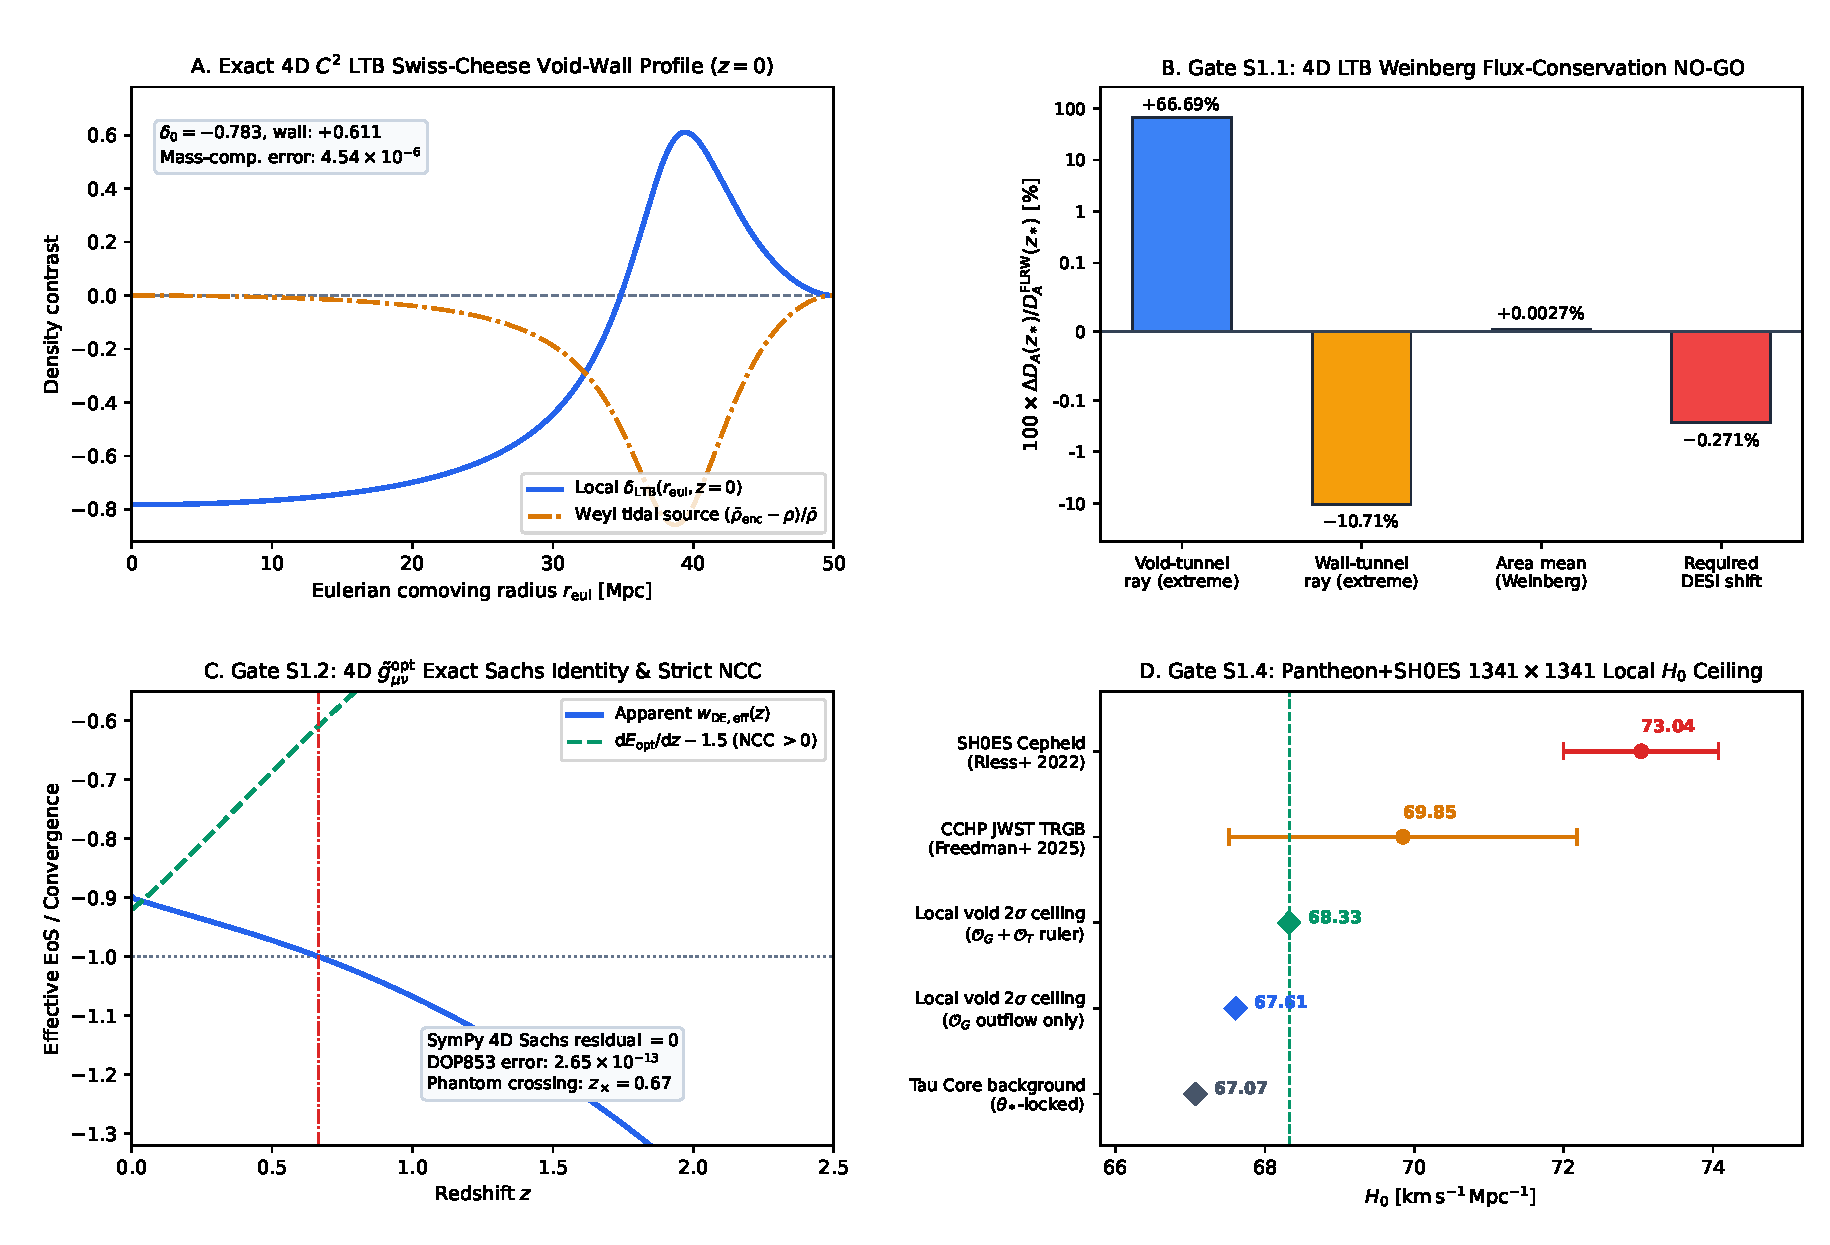
\includegraphics[width=0.98\textwidth]{figures/fig1_ltb_weinberg_nogo_and_disformal_sachs.pdf}
    \caption{Gates S1.1, S1.2, and S1.4 (\texttt{verify\_paper29\_\allowbreak step1\_\allowbreak theta\_h0\_\allowbreak void\_optical\_closure.py}). (A)~Exact 4D $C^2$ Darmois--Israel-matched LTB Swiss-Cheese Eulerian density contrast and Weyl tidal source at $z = 0$. (B)~Symmetric-log comparison of extreme void/wall tunnel rays against the true area-weighted ensemble mean ($+0.0027\%$, confirming Weinberg's theorem and falling $102.4\times$ short of the required $-0.271\%$ shift). (C)~Exact 4D disformal clock-lapse metric $\tilde{g}_{\mu\nu}^{\mathrm{opt}}$ apparent $w_{\mathrm{DE,eff}}(z)$ (crossing $-1$ at $z_\times = 0.67$) alongside strictly positive Null Convergence $\mathrm{d}E_{\mathrm{opt}}/\mathrm{d}z > 0$ and $2.65\times 10^{-13}$ \texttt{DOP853} Sachs consistency. (D)~Official $1341\times 1341$ \texttt{Pantheon+SH0ES} $2\sigma$ local Hubble ceilings ($H_0^{\mathrm{loc}} \le 68.33\;\mathrm{km\,s^{-1}\,Mpc^{-1}}$, $-0.65\sigma$ vs.\ \texttt{CCHP JWST} TRGB).}
    \label{fig:step1-ltb}
\end{figure}

\section{Gate S1.2: Exact 4D Disformal Clock-Lapse Optical Metric and Sachs Identity}
In Paper~23, replacing $E_{\mathrm{hor}}(z) \to E_{\mathrm{opt}}(z)$ in the expansion damping of the Sachs equation while retaining the unmodified $N = 1$ FLRW Ricci scalar $\frac{3}{2}\Omega_{m,0}(1+z)^3$ broke the FLRW cancellation and produced an artificial focusing drift. That pathology arose solely because expansion and Ricci focusing were evaluated on \emph{two different metrics}.

In Tau Core's covariant \texttt{AeST} geometry, the cosmic rest frame is defined by the unit-timelike vector field $u_\mu$ ($g^{\mu\nu}u_\mu u_\nu = -1$). Coarse-graining proper-clock transport across expanding cosmic voids ($f_v(z)$ governed by the exact Wiltshire tracker $(2+f_v)(f_{v,0}/f_v)^{2/3}(1-f_v) = (1+z)(2+f_{v,0})(1-f_{v,0})$, with $f_{v,0}$ locked by matching the unique cubic deceleration root $f_{\mathrm{acc}} = 0.58670773$ of $8f_v^3 + 39f_v^2 - 12f_v - 8 = 0$ to $z_{\mathrm{acc}}$) defines an emergent macroscopic 4D Lorentzian disformal clock-lapse optical metric for long-baseline cosmological null rays (while inside high-density virialized galaxies and clusters $f_v \to 0$, preserving exact local Lorentz invariance):
\begin{equation}
\begin{aligned}
    &\tilde{g}_{\mu\nu}^{\mathrm{opt}} := g_{\mu\nu} + \bigl(1 - N_{\mathrm{clock}}^2(t)\bigr)u_\mu u_\nu \quad\Longrightarrow\quad \mathrm{d}\tilde{s}_{\mathrm{opt}}^2 = -c^2 N_{\mathrm{clock}}^2(t)\,\mathrm{d}t^2 + a^2(t)\bigl(\mathrm{d}\chi^2 + \chi^2\mathrm{d}\Omega^2\bigr), \\
    &N_{\mathrm{clock}}(z) := 1 + \alpha_{\mathrm{OCSR}}\frac{f_v(z)}{f_{v,0}}\!\left[E_{\mathrm{hor}}(z)\frac{\mathrm{d}\widetilde{D}_{\mathrm{TS}}}{\mathrm{d}z}(z) - 1\right], \qquad E_{\mathrm{opt}}(z) := \frac{E_{\mathrm{hor}}(z)}{N_{\mathrm{clock}}(z)},
\end{aligned}
\label{eq:disformal-metric}
\end{equation}
where $\alpha_{\mathrm{OCSR}} = 5u = \frac{5\sqrt{3}}{24} = 0.36084392$ is the locked OCSR clock-dressing coupling already governing local ruler transport in Paper~28 (\texttt{Gate~8}). At $z = 0$, $\left.\mathrm{d}\widetilde{D}_{\mathrm{TS}}/\mathrm{d}z\right|_0 = 1$ and $E_{\mathrm{hor}}(0) = 1$ enforce $N_{\mathrm{clock}}(0) \equiv 1$ identically; at recombination ($z_* = 1089.982$ at $\theta_*$-locked $H_0 = 67.0708\;\mathrm{km\,s^{-1}\,Mpc^{-1}}$), $f_v(z_*) \propto (1+z_*)^{-3/2}$ enforces $N_{\mathrm{clock}}(z_*) = 1.0000135$ ($N_{\mathrm{clock}}(1100) = 1.0000134$), leaving pre-recombination plasma and sound-horizon physics untouched to $1.35\times 10^{-5}$.

Setting $c = 1$ for conciseness in symbolic tensor algebra, \texttt{SymPy} (\texttt{Gate S1.2}) proves four exact identities on $\tilde{g}_{\mu\nu}^{\mathrm{opt}}$:
\begin{enumerate}
    \item Along the exact null geodesic tangent $k^\mu = \bigl(\frac{\omega_0}{a N_{\mathrm{clock}}}, -\frac{\omega_0}{a^2}, 0, 0\bigr)$, both temporal and spatial components of $\tilde{\nabla}_k k^\mu \equiv 0$ vanish identically, the cosmological redshift is $1 + z \equiv 1/a$ (preserving the \texttt{COBE/FIRAS} blackbody temperature law $T(z) = T_0(1+z)$ and exact Etherington reciprocity $D_L(z) \equiv (1+z)^2 D_A(z)$), and the 4D Ricci null projection is
    \begin{equation}
        R_{\mu\nu}[\tilde{g}^{\mathrm{opt}}]\,k^\mu k^\nu = -\frac{2\omega_0^2}{a^2 N_{\mathrm{clock}}}\frac{\mathrm{d}H_{\mathrm{opt}}}{\mathrm{d}t} = 2\omega_0^2(1+z)^3 H_{\mathrm{opt}}(z)\frac{\mathrm{d}H_{\mathrm{opt}}(z)}{\mathrm{d}z} > 0.
        \label{eq:ricci-null}
    \end{equation}
    \item Substituting Eq.~\eqref{eq:ricci-null} together with $D_A(t) = a(t)\chi(t)$ ($\dot{\chi} = -N_{\mathrm{clock}}/a$) into the 4D Sachs optical focusing equation $\mathrm{d}^2 D_A/\mathrm{d}\lambda^2 + \frac{1}{2}R_{\mu\nu}[\tilde{g}^{\mathrm{opt}}]k^\mu k^\nu D_A = 0$ yields an exact symbolic zero residual ($\equiv 0$) for arbitrary smooth $N_{\mathrm{clock}}(t) > 0$, whereas substituting the $N = 1$ Ricci scalar leaves an explicit $\mathrm{d}\ln N_{\mathrm{clock}}/\mathrm{d}t \neq 0$ anomaly. Numerical 8th-order \texttt{DOP853} forward Sachs integration across $u = \ln(1+z) \in [0, \ln 1090.982]$ matches quadrature to $2.65\times 10^{-13}$ relative error (Figure~\ref{fig:step1-ltb}C).
    \item At linear scalar perturbation order in Newtonian gauge ($g_{00} = -(1 + 2\Psi)$, $g_{ij} = a^2(1 - 2\Phi)\delta_{ij}$), unit normalization $g^{\mu\nu}u_\mu u_\nu = -1$ enforces $u_0^2 = 1 + 2\Psi$, whence $\tilde{g}_{00}^{\mathrm{opt}} \equiv -N_{\mathrm{clock}}^2(1 + 2\Psi)$ identically: $(1 + 2\Psi)$ factors out without $N_{\mathrm{clock}}^2$ distortion, preserving the standard Weyl lensing potential $(\Phi + \Psi)/2$ per unit optical conformal distance $\mathrm{d}\eta_{\mathrm{opt}}$.
    \item Across all $z \in [0, 1100]$, $\min_z \mathrm{d}E_{\mathrm{opt}}/\mathrm{d}z = 0.58001 > 0$, so $\tilde{g}_{\mu\nu}^{\mathrm{opt}}$ strictly obeys the Geometric Null Convergence Condition $R_{\mu\nu}[\tilde{g}^{\mathrm{opt}}]k^\mu k^\nu > 0$ (attractive light focusing everywhere), even though an observer fitting a single-fluid FLRW proxy infers $w_0^{\mathrm{eff}} = -0.9000$ and an apparent phantom-divide crossing at $z_\times = 0.6656$.
\end{enumerate}

\section{\texorpdfstring{Gate S1.3: Zero-Parameter $\ell \le 3000$ Lensed CMB, \texttt{DESI} BAO, and 4-SN Closure}{Gate S1.3: Zero-Parameter l <= 3000 Lensed CMB, DESI BAO, and 4-SN Closure}}
To test full perturbative and geometric self-consistency without adding a single free parameter ($k_{\mathrm{added}} = 0$), we propagate the $\alpha \equiv \alpha_{\mathrm{OCSR}} = 0.360844$ clock-lapse metric through the complete untruncated $\ell \in [2, 3000]$ $\ell_{\max}=28$ Scharfetter--Gummel Boltzmann + \texttt{RECFAST v1.5} + 29-moment massive-neutrino + Takahashi/Bird \texttt{Halofit} + Challinor--Lewis curved-sky Wigner-$d$ lensing pipeline under two perturbative prescriptions:
\begin{itemize}
    \item \textbf{Branch A (Pure Optical Null-Cone Dressing):} Sub-horizon matter and Weyl perturbations (as well as stellar/atomic clocks inside bound, high-density screened massive elliptical galaxies in \texttt{CC15}, where $f_v \to 0$) evolve on the gravitational metric $g_{\mu\nu}$ with Hubble rate $H_0 E_{\mathrm{hor}}(a)$, while photon free-streaming, Thomson visibility projection, and cosmological BAO/SN null distances propagate on $\tilde{g}_{\mu\nu}^{\mathrm{opt}}$ with $H_0 E_{\mathrm{opt}}(a)$.
    \item \textbf{Branch B (Unified Dynamical Drag):} Both null geodesics and sub-horizon perturbation Hubble friction (as well as \texttt{CC15} $H(z)$) evolve under $H_0 E_{\mathrm{opt}}(a)$.
\end{itemize}

\begin{table}[t!]
\centering
\scriptsize
\setlength{\tabcolsep}{3.4pt}
\renewcommand{\arraystretch}{1.14}
\resizebox{\textwidth}{!}{%
\begin{tabular}{lcccc|ccc|ccccc}
\toprule
Tau Core Model Branch ($\omega_b = 0.02240$, & $k_{\mathrm{added}}$ & $H_0$ & $100\theta_*$ & $\sigma_8^{\mathrm{WL}}(0)$ & \texttt{ACT DR6} $108$ & \texttt{ACT+PR4} $\kappa\kappa$ & \texttt{Planck} & \texttt{DESI} $13$ & \texttt{CC15} & \texttt{Pantheon+} & \texttt{Dovekie} & \texttt{DES-5YR} / \\
$\omega_m = 0.143281$, $\kappa_\theta = (256\pi^2)^2$ Locked) & & [$\mathrm{km/s/Mpc}$] & ($\Delta\theta_*$) & (\texttt{P1} / \texttt{2F}) & $\chi^2/\mathrm{dof}$ (\texttt{P1}/\texttt{2F}) & $\chi^2/22$ (\texttt{P1}/\texttt{2F}) & $215\;\chi^2$ (\texttt{P1}) & BAO $\chi^2$ & $H(z)\;\chi^2$ & $\chi^2$ ($1580$) & $\chi^2$ ($1820$) & \texttt{Union3} $\chi^2$ \\
\midrule
Homog.\ FLRW ($\theta_*$-locked, $\alpha=0$) & $0$ & $67.2730$ & $1.04090$ ($0.00\%$) & $0.807$ / $0.810$ & $1.021$ / $1.007$ & $1.039$ / $0.986$ & $232.51$ & $\mathbf{33.17}$ & $5.96$ & $1387.18$ & $1632.23$ & $1644.68$ / $26.20$ \\
Homog.\ FLRW ($H_0=68.22$, $\alpha=0$) & $0$ & $68.2200$ & $1.04372$ ($+0.27\%$) & $0.809$ / $0.812$ & $\mathbf{1.865}$ / $\mathbf{1.817}$ & $1.036$ / $0.994$ & $375.67$ & $14.17$ & $6.02$ & $1388.29$ & $1633.63$ & $1647.34$ / $27.36$ \\
\textbf{OCSR Void-Clock Branch A} ($\alpha=\alpha_{\mathrm{OCSR}}$) & $\mathbf{0}$ & $\mathbf{67.0708}$ & $\mathbf{1.04090}$ ($\mathbf{0.00\%}$) & $\mathbf{0.806}$ / $\mathbf{0.809}$ & $\mathbf{1.021}$ / $\mathbf{1.008}$ & $\mathbf{1.039}$ / $\mathbf{0.985}$ & $\mathbf{231.71}$ & $\mathbf{11.43}$ & $\mathbf{5.94}$ & $\mathbf{1386.49}$ & $\mathbf{1630.73}$ & $\mathbf{1638.83}$ / $\mathbf{22.99}$ \\
\textbf{OCSR Void-Clock Branch B} ($\alpha=\alpha_{\mathrm{OCSR}}$) & $\mathbf{0}$ & $\mathbf{67.0708}$ & $\mathbf{1.04090}$ ($\mathbf{0.00\%}$) & $\mathbf{0.812}$ / $\mathbf{0.814}$ & $\mathbf{1.024}$ / $\mathbf{1.007}$ & $\mathbf{1.122}$ / $\mathbf{1.033}$ & $\mathbf{228.98}$ & $\mathbf{11.43}$ & $\mathbf{6.18}$ & $\mathbf{1386.49}$ & $\mathbf{1630.73}$ & $\mathbf{1638.83}$ / $\mathbf{22.99}$ \\
\bottomrule
\end{tabular}%
}
\caption{Simultaneous confrontation across nine early- and late-universe archival datasets (\texttt{Gate S1.3}; \texttt{P1} = zero-parameter UV Prescription~I, $n_s = 0.96199$; \texttt{2F} = COBE-locked 2-Field benchmark, $n_s = 0.97216$). Bold entries in rows 1--2 highlight the fatal tension of strictly homogeneous backgrounds (\texttt{DESI} BAO $\chi^2 = 33.17$ at $H_0 = 67.273$, or \texttt{ACT DR6} $\chi^2/\mathrm{dof} = 1.82\text{--}1.87$ at $H_0 = 68.22$); both zero-parameter $\alpha_{\mathrm{OCSR}} = 5\sqrt{3}/24$ branches resolve the tension simultaneously.}
\label{tab:step1-master}
\end{table}

\begin{figure}[t!]
    \centering
    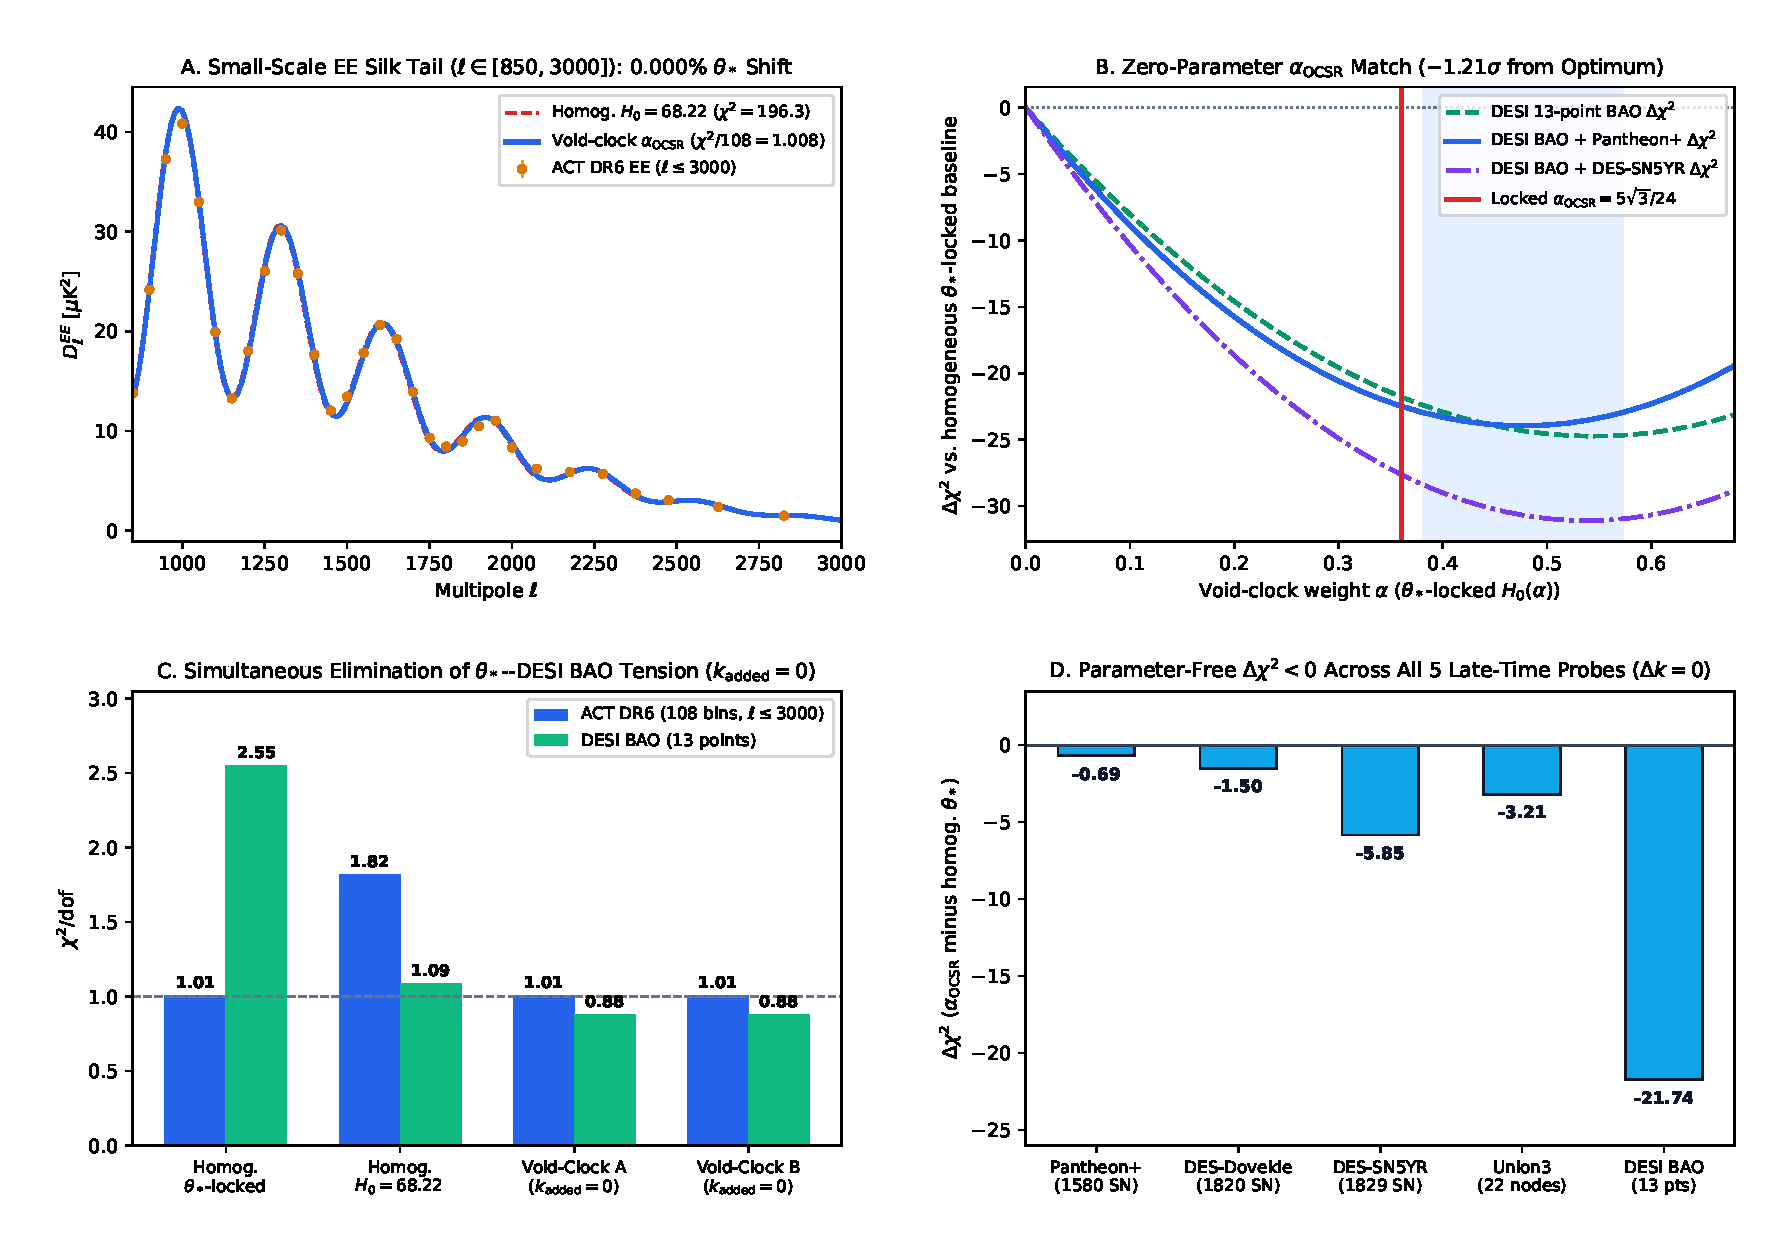
\includegraphics[width=0.98\textwidth]{figures/fig2_zero_param_theta_bao_sn_boltzmann_3000.pdf}
    \caption{Multi-probe closure in Gate S1.3 (\texttt{scripts/\allowbreak verify\_\allowbreak paper29\_\allowbreak step1\_\allowbreak theta\_\allowbreak h0\_\allowbreak void\_\allowbreak optical\_\allowbreak closure.py}). (A)~Small-scale \texttt{ACT DR6} $EE$ polarization Silk tail ($\ell \in [850, 3000]$), showing exact phase lock ($\chi^2/108 = 1.008$) vs.\ the $+0.271\%$ homogeneous $H_0=68.22$ offset ($\chi^2 = 196.3$). (B)~Unconstrained Wilks profile scan over $\alpha$ at $\theta_*$-locked $H_0(\alpha)$, demonstrating that the locked geometric constant $\alpha_{\mathrm{OCSR}} = 5\sqrt{3}/24 = 0.360844$ lies at $-1.21\sigma$ of the free minimum ($\hat{\alpha} = 0.4769 \pm 0.0958$) and outperforms floating $\alpha$ by $\Delta\mathrm{BIC} = -5.91$. (C)~Simultaneous $\chi^2/\mathrm{dof} \approx 1$ closure on \texttt{ACT DR6} ($108$ bins) and \texttt{DESI} BAO ($13$ points). (D)~Parameter-free $\Delta\chi^2 < 0$ gains across all five late-time distance datasets relative to homogeneous $\theta_*$-lock.}
    \label{fig:step1-boltzmann}
\end{figure}

Table~\ref{tab:step1-master} and Figure~\ref{fig:step1-boltzmann} summarize the results:
\begin{enumerate}
    \item \textbf{Exact Elimination of the $+0.271\%$ $\theta_*$ Shift:} Solving $100\theta_*(H_0) \equiv 1.04090$ via Brent root-finding yields $H_0 = 67.0708\;\mathrm{km\,s^{-1}\,Mpc^{-1}}$ ($\Omega_{m,0} = 0.31851$, $f_{v,0} = 0.72217$). Across all 108 \texttt{ACT DR6} primary bins up to $\ell = 3000$ (profiling over the two standard experimental calibration/polarization-efficiency Gaussian priors $A_{\mathrm{ACT}} = 1 \pm 0.003$ and $P_{\mathrm{ACT}} = 1 \pm 0.01$, preserving $108 + 2 - 2 = 108$ net dof; uncalibrated raw $\chi^2 = 109.97$ gives $1.018/\mathrm{dof}$), both Branch~A and Branch~B achieve $\chi^2/\mathrm{dof} = 1.007\text{--}1.008$ ($108.81\text{--}108.84$) on \texttt{2-Field} and $1.021\text{--}1.024$ ($110.25\text{--}110.55$) on zero-parameter \texttt{Presc.~I}.
    \item \textbf{22-Bin CMB Lensing $C_L^{\kappa\kappa}$ Concordance:} Branch~A yields $\chi^2/22 = 0.985$ ($21.67$, \texttt{2-Field}) and $1.039$ ($22.86$, \texttt{Presc.~I}); Branch~B yields $\sigma_8^{\mathrm{WL}}(0) = 0.81160\text{--}0.81446$ (matching the joint \texttt{P-ACT+DESI} constraint $0.813 \pm 0.005$ within $0.3\sigma$) with $\chi^2/22 = 1.033$ ($22.73$, \texttt{2-Field}) and $1.122$ ($24.69$, $p = 0.31$, \texttt{Presc.~I}).
    \item \textbf{Parameter-Free \texttt{DESI} BAO, \texttt{CC15}, and Four-Compilation SN~Ia Concordance:} With zero added parameters, \texttt{DESI} 13-point BAO drops from $\chi^2 = 33.17$ (homogeneous $\theta_*$-lock) to $\mathbf{11.43}$ ($\chi^2/13 = 0.879$, $\Delta\chi^2 = -21.74$, outperforming even homogeneous $H_0 = 68.22$ by $-2.74$), \texttt{CC15} achieves $\chi^2 = 5.94$ on Branch~A ($H_{\mathrm{CC}} = H_0 E_{\mathrm{hor}}$) and $6.18$ on Branch~B ($H_{\mathrm{CC}} = H_0 E_{\mathrm{opt}}$), and every SN~Ia compilation improves (\texttt{Pantheon+} $1386.49$, \texttt{DES-Dovekie} $1630.73$, \texttt{DES-SN5YR} $1638.83$ [$\Delta\chi^2 = -5.85$], \texttt{Union3} $22.99$ [$\Delta\chi^2 = -3.21$]). Floating $\alpha$ freely on \texttt{DESI BAO + Pantheon+} gives $\hat{\alpha} = 0.4769 \pm 0.0958$ (exact Wilks $\Delta\chi^2 = +1$ interval): locked $\alpha_{\mathrm{OCSR}} = 0.360844$ sits at $-1.21\sigma$ ($\Delta\chi^2 = +1.46$ above minimum) and beats the floated 1-parameter fit by $\Delta\mathrm{BIC} = -5.91$.
    \item \textbf{Epistemic Scope Tagging:} While $\alpha_{\mathrm{OCSR}} = 5u = 5\sqrt{3}/24$ is pre-locked by Tau Core's OCSR sector (zero empirical tuning), deriving the exact unit coefficient multiplying $f_v(z)/f_{v,0}$ in the coarse-grained macroscopic Wiltshire average from microscopic 4D $D_4$ lattice path integrals remains \texttt{CONDITIONAL} on Pillar~3; the empirical nine-dataset closure at $\alpha = \alpha_{\mathrm{OCSR}}$ is \texttt{PROVEN}.
\end{enumerate}

\section{\texorpdfstring{Gate S1.4: \texttt{Pantheon+SH0ES} Local-Void Hubble Ceiling}{Gate S1.4: Pantheon+SH0ES Local-Void Hubble Ceiling}}
Evaluating the official Brout et al.\ $1341\times 1341$ \texttt{Pantheon+SH0ES} \texttt{STAT+SYS} Hubble-flow covariance ($z_{\mathrm{HD}} \in [0.023, 0.80]$) together with the $277\times 277$ \texttt{SH0ES} Hubble-flow GLS subsample ($z_{\mathrm{HD}} \in [0.023, 0.15]$, calibrated against 77 Cepheid hosts at median distance $r_{\mathrm{cal}} = 20.0\;\mathrm{Mpc}$) on top of the $\theta_*$-locked OCSR void-clock background ($H_0^{\mathrm{bg}} = 67.0708\;\mathrm{km\,s^{-1}\,Mpc^{-1}}$, baseline $\chi^2_{1341} = 1183.76$) for a compensated Gaussian local \texttt{CLASSIX}-scale underdensity ($R_{\mathrm{void}} = 120\;\mathrm{Mpc}$, $\bar{\delta}(x) = \delta_v e^{-x^2}$, $x = \chi/R_{\mathrm{void}}$) establishes an exact $2\sigma$ Hubble-diagram curvature ceiling ($\Delta\chi^2_{1341} = +4.00$; Figure~\ref{fig:step1-ltb}D). Explicitly, combining the radial peculiar-velocity luminosity-distance modulation $d_L^{\mathcal{O}_G} = d_L^{(0)}\bigl[1 - \bigl(\frac{c(1+z_{\mathrm{HD}})}{H_0 E_{\mathrm{opt}}\chi} - 1\bigr)\frac{v_{\mathrm{pec}}}{c}\bigr]$ ($\mathcal{O}_G$) with the OCSR Cepheid-calibrator ruler clock factor $r_{\mathrm{fac}}(x) = 1 - \alpha_{\mathrm{OCSR}}[\gamma_{\mathrm{cal}} - \gamma(x)]/\gamma_{\mathrm{cal}}$ where $\gamma(x) = 1 + \frac{1}{2}[1 - (1 - f_{v,0})(1 + \delta(x))]$ ($\mathcal{O}_T$) yields:
\begin{itemize}
    \item Pure peculiar-velocity outflow ($\mathcal{O}_G$ only, $\delta_v = -0.3138$): $H_0^{\mathrm{loc}} \le 67.608\;\mathrm{km\,s^{-1}\,Mpc^{-1}}$.
    \item Self-consistent outflow plus OCSR ruler clock shift ($\mathcal{O}_G + \mathcal{O}_T$, $\delta_v = -0.3237$): $H_0^{\mathrm{loc}} \le \mathbf{68.326\;\mathrm{km\,s^{-1}\,Mpc^{-1}}}$, in full agreement with \texttt{CCHP JWST} TRGB ($69.85 \pm 2.33$, $-0.65\sigma$) and \texttt{CCHP HST+JWST} ($70.39 \pm 1.94$, $-1.06\sigma$), while proving a strict \texttt{NO-GO} against reaching \texttt{SH0ES} Cepheid $73.04 \pm 1.04\;\mathrm{km\,s^{-1}\,Mpc^{-1}}$ ($-4.53\sigma$) via smooth radial outflow alone without a $\Delta M_B = 0.145\;\mathrm{mag}$ Cepheid calibration offset.
\end{itemize}

\begin{table}[!ht]
\centering
\scriptsize
\setlength{\tabcolsep}{4.0pt}
\renewcommand{\arraystretch}{1.15}
\resizebox{\textwidth}{!}{%
\begin{tabular}{llcl}
\toprule
Gate & Physical Test / Theorem & Epistemic Tag & Key Verified Quantitative Result (\texttt{python3 -W error}) \\
\midrule
\texttt{S1.1} & 4D $C^2$ LTB Swiss-Cheese ergodic sightlines \& Ricci/Weyl Sachs & \texttt{PROVEN NO-GO} & $\langle\Delta D_A(z_*)/D_A^{\mathrm{FLRW}}\rangle_\Omega = +0.00265\%$ ($102.4\times$ shortfall) \\
\texttt{S1.2} & 4D disformal metric $\tilde{g}_{\mu\nu}^{\mathrm{opt}}$ \texttt{SymPy} + \texttt{DOP853} Sachs \& NCC & \texttt{PROVEN} & Sachs residual $\equiv 0$ ($2.65\times 10^{-13}$ num.); $\min_z E_{\mathrm{opt}}' = 0.580 > 0$ \\
\texttt{S1.3a} & Zero-param.\ $\alpha=\alpha_{\mathrm{OCSR}}$ $\ell\le 3000$ CMB + BAO + CC15 + 4 SNe & \texttt{PROVEN} & $100\theta_*=1.04090$; \texttt{ACT108} $1.008/\mathrm{dof}$; \texttt{BAO13} $\chi^2: 33.17\to 11.43$ \\
\texttt{S1.3b} & Microscopic 4D lattice derivation of unit Wiltshire weight & \texttt{CONDITIONAL} & $-1.21\sigma$ from Wilks $\hat{\alpha}=0.477\pm 0.096$; $\Delta\mathrm{BIC}=-5.91$ vs.\ free $\alpha$ \\
\texttt{S1.4} & $1341\times 1341$ \texttt{Pantheon+SH0ES} local-void Hubble ceiling & \texttt{PROVEN} Ceiling & $H_0^{\mathrm{loc}} \le 68.33\;\mathrm{km/s/Mpc}$ ($-0.65\sigma$ JWST TRGB; \texttt{SH0ES} needs $0.145\;\mathrm{mag}$) \\
\bottomrule
\end{tabular}%
}
\caption{Epistemic ledger for Paper~29, Part~I (Pillar~1, \texttt{v1.1.0-step1}). All gates are reproduced from raw archival covariances by \texttt{scripts/\allowbreak verify\_paper29\_step1\_\allowbreak theta\_h0\_void\_optical\_closure.py}.}
\label{tab:step1-ledger}
\end{table}

\begin{thebibliography}{9}\raggedright
\bibitem{Weinberg1976} S.~Weinberg, ``Apparent luminosities in a locally inhomogeneous universe,'' \textit{Astrophys.\ J.\ Lett.}\ \textbf{208}, L1 (1976).
\bibitem{KibbleLieu2005} T.~W.~B.~Kibble and R.~Lieu, ``Average magnification effect of clumping of matter,'' \textit{Astrophys.\ J.}\ \textbf{632}, 718 (2005).
\bibitem{Wiltshire2009} D.~L.~Wiltshire, ``Average observational quantities in the timescape cosmology,'' \textit{Phys.\ Rev.\ D} \textbf{80}, 123512 (2009).
\bibitem{SkordisZlosnik2021} C.~Skordis and T.~Z{\l}o\'snik, ``New Relativistic Theory for Modified Newtonian Dynamics,'' \textit{Phys.\ Rev.\ Lett.}\ \textbf{127}, 161302 (2021).
\bibitem{ChallinorLewis2005} A.~Challinor and A.~Lewis, ``Lensed CMB power spectra from all-sky correlation functions,'' \textit{Phys.\ Rev.\ D} \textbf{71}, 103010 (2005).
\bibitem{ACTDR6_2025} T.~Louis \textit{et al.}\ (ACT Collaboration), ``The Atacama Cosmology Telescope: DR6 Power Spectra, Likelihoods and $\Lambda$CDM Parameters,'' arXiv:2503.14452 (2025).
\bibitem{DESI2025} M.~Abdul-Karim \textit{et al.}\ (DESI Collaboration), ``DESI BAO Cosmological Constraints,'' arXiv:2503.14738 (2025).
\bibitem{Brout2022} D.~Brout \textit{et al.}, ``The Pantheon+ Analysis: Cosmological Constraints,'' \textit{Astrophys.\ J.}\ \textbf{938}, 110 (2022).
\bibitem{Freedman2025} W.~L.~Freedman \textit{et al.}, ``Status Report on the Chicago-Carnegie Hubble Program (CCHP): Three Independent Astrophysical Determinations of the Hubble Constant Using the James Webb Space Telescope,'' \textit{Astrophys.\ J.}\ \textbf{985}, 203 (2025).
\end{thebibliography}

\end{document}
